%\section{Company-wide}
\section{Organization and employees}
\label{sec:companywide}
The company is divided into two departments, Product \& Sales (P\&S) and Research \& Development (R\&D). The focus of the P\&S department is mainly customer contact, requirements and testing. The R\&D department mainly focuses on topics regarding design and implementation. From these teams we have created cross functional teams with a specific task. These teams have developed during the project to focus on different tasks as the projects needs have changed, see more under \ref{sec:companywide:subsection:cft} %expand this part 
\subsection{Roles}
\begin{figure}[ht]
    \centering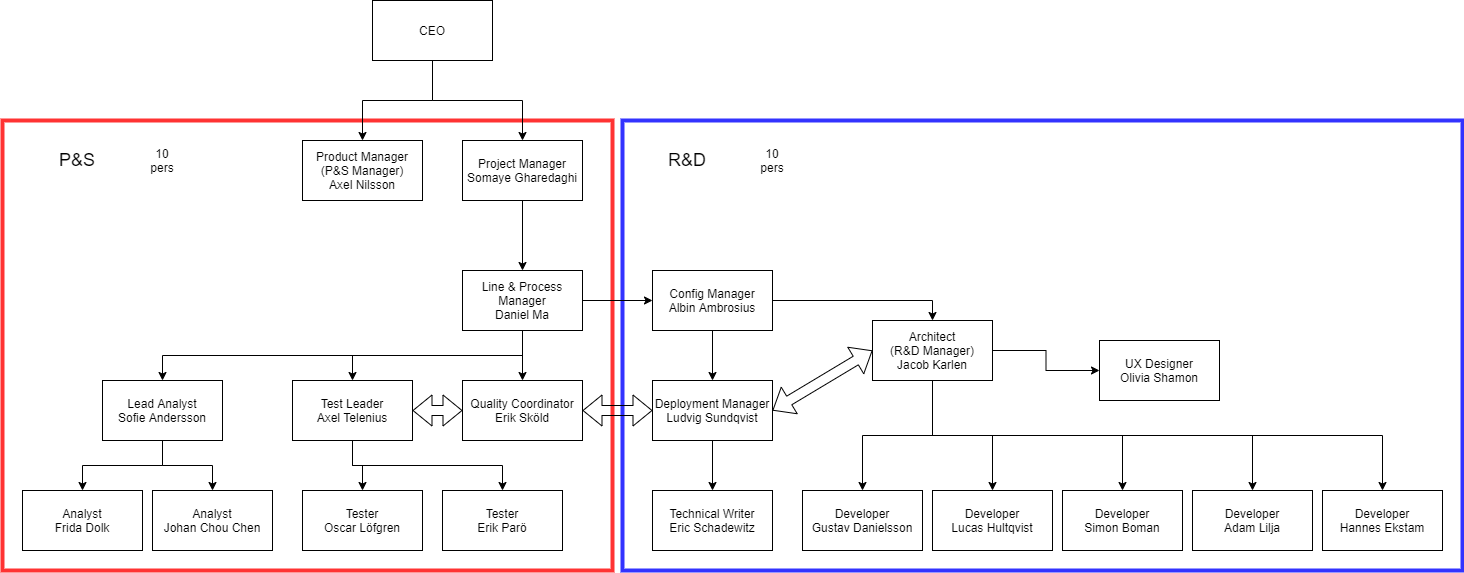
\includegraphics[width=1 \linewidth]{figures/company flowchart.png}
    \caption{Company Flowchart (first half of the project)}
    \label{fig:example2}
\end{figure}


%description of each role in details from teams and their names
\subsubsection*{Product Manager – Axel Nilsson}
A strategic product owner is to be the link between the customer and the developers. This means handling the product backlog and trying to prioritize requirements in the best way possible to match customer needs. Also, creating a vision for the product so the whole team knows what we are working towards. 

\subsubsection*{Project Manager – Somaye Gharedaghi} 
Breaking down the work by creating project plan, making sure that everyone has something to do in a timely manner, making sure that everyone has the view of the plan to know how they can contribute and collaborate, running the meetings, and keeping the project organized. These all are achievable through having either regular managers meetings or one by one, keeping in touch with managers, and listening to their concerns. Setting agenda for meetings according to following up the progress of the project and managers’ concerns. As well as presenting the weekly report to the CEO at CEO Meeting and sending weekly status reports to the CEO, the consulting supervisors, the examiner, and to the employees of the company. 

\subsubsection*{Line \& Process Manager – Daniel Ma}
Ensures good working environments and sees to it that everyone feels involved and content. Handles formal communication with the company leadership. Develops and handles the company's processes along with the Quality coordinator.

\subsubsection*{Lead Analyst - Sofie Andersson} 
Main responsibility to have contact with our customer and understand what they want from our system and what they need. Also responsible for making progress in the analyst work and communicate to the manager group about it.  

The analyst team is responsible to define requirements and user stories so that the development group knows what to do and have customer meetings.  

\subsubsection*{Analysts - Frida Dolk \& Johan Chou Chen} 
Analysts are responsible together with the Lead analyst to structure the work with the customer and align the customer needs with the rest of the company. Shall understand customers desires and put down these into requirements, in a concrete, detailed and organized way and deliver to the developer team. 

\subsubsection*{Test Leader - Axel Telenius} 
Handling testing operations towards customer, following up work by test team, and coordinate with quality coordinator to ensure software meets specifications from testing point of view.

\subsubsection*{Testers - Oscar Löfgren \& Erik Parö}

Testers assist the test leader with the test, assist the test leader with coming up with an explicit plan for the testing and reporting of the test results. They are responsible for creating relevant test documents and make sure to follow them. 

\subsubsection*{Quality Coordinator - Erik Sköld} 
Measures and monitors the product quality and initiates necessary changes of product and process. Responsible for explicated plan for quality assurance. Works together with the testing team on the software quality assurance plan. Reviews decisions on code conventions, test tools and reporting. Collects means of quality work, verifies traceability and makes sure the work fit together. 

\subsubsection*{Configuration Manager – Albin Ambrosius} 
To ensure that all tool, software or hardware, are being utilized and that the progress is being tracked. Will see to it that everyone is notified of changes in the tools or assets that we create.  Handling the set-ups for new tools and communicates with both the development team and company leadership through R\&D reports.  

\subsubsection*{Architect – Jacob Karlén} 
Specifies and decides on high-level architecture, target environment and components to be used. Ensures that functional and non-functional requirements are met and coordinates with other teams on technical matters. Responsible for the Architecture Notebook.  

\subsubsection*{R\&D Manager – Ludvig Sundqvist}
Responsible for scheduling, sending out agendas and moderating R\&D meetings and coordinating the work within the department.  

\subsubsection*{UX Designer – Olivia Shamon} 
Specializes in setting targets and realizing the user experience of the system. Creates prototypes of the system for the developers.  

\subsubsection*{Deployment Manager – Ludvig Sundqvist}
Makes sure the product is made available to the customer and plan and prepare for continuous deployment. Works as a middleman between the testers and developers, works closely with the architect and test leader. Is the responsible manager for Docker, Git and containers. 

\subsubsection*{Technical Writer – Eric Schadewitz} 
Ensures that the output of the project is accessible to our customer. Produces instructions on how to use the system the way it was developed to be used. Also documents suggestions for further development. 

\subsubsection*{Developers – Gustav Danielsson, Lucas Hultqvist, Simon Boman, Adam Lilja \& Hannes Ekstam Ljusegren} 
Have the main responsibility of realizing requirements into functions of the software solution. 

\subsection{Cross-functional teams}
\label{sec:companywide:subsection:cft}
The company is further divided into three cross functional teams (hereinafter CFT), with members from both departments and with different roles. The idea with the CFTs is to speed up development and still ensure that the right competence is present in each team. One key area of the project is the requirement specification. Expertise of this area is carried by the company's analysts, and thus a decision was made to have one analyst in each CFT so that this knowledge is dispersed throughout the whole company. During the pre-study phase, the CFTs have each developed a prototype which is an example of what the responsibilities of the CFTs are. The members and structures of the CFTs may change during the development phase (between iterations) depending on customer needs, course requirements, or any other reasonable reason. 

The second iteration of CFTs consisted of members from all over the company and had three focus areas: back-end development, patient overview development, and patient dashboard development. As the project went on we discovered that this iteration of CFTs was not the most optimal option for our company and decided to change the teams up for the next iteration. The next iteration of CFTs got a more clear goal, the first one would be developer-heavy and focus on completing the issues with the highest rank. The second team would focus on UX-design and provide the development team with prototypes when needed and also test the implemented component to verify that they work in the intended way UX-wise. The last team would focus on testing and quality, with tasks such as implementing a pipeline in GitLab with automated tests and accepting merge-requests.

%moved below part to Processes section (whatever related to communication and processes)

%After the toll-gate, reasonably large tasks within CFTs shall be listed as cards on the Gitlab board for that specific team. Members of the CFT shall assign their name to the tasks that they will be working on. As well as this, the burndown chart in Git will be updated over the task selection and done.

%Each Friday the team leaders for each CFT will meet with the person responsible for the status reports to update on progress. This achieves two things: first, the progress of each CFT can be documented in the status reports; secondly, the progress can be analyzed and compared with the set milestones to see if the teams are on track or if something needs to change in order to reach the milestones in time. 

%\subsection{General} 
